

\section{Methods}

% brief introduction of the k-armed bandit problem and previous algorithms.
\subsection{Related work}
% overview of the main solutions proposed in the literature from a computational perspective.
There exists various flavours of this problem, with the simplest having a stationary reward distribution, while the more challening ones have have \textit{concept drift}, where the reward distribution changes over time.
Over the years, several algorithms have been proposed, alongside with their theoretical guarantees. In this regard, Thompson sampling is a popular algorithm that has been shown to achieve near-optimal regret bounds in the stochastic setting \cite{agrawalAnalysisThompsonSampling2012}, which 
a Bayesian approach  the idea of maintaining a posterior distribution over the reward probabilities of the actions, and selecting actions according to the posterior distribution. Another popular algorithm is the Upper Confidence Bound (UCB) algorithm, which has been shown to achieve near-optimal
regret bounds in the adversarial setting \cite{auerFinitetimeAnalysisMultiarmed2002}. The algorithm is based on the idea of maintaining an upper confidence bound on the reward probabilities of the actions, and selecting actions according to the upper confidence bound.
\\
% outline of lack of bio-realism and what we currently know about how the brain might solve this task.
Despite the success of these algorithms in solving the k-armed bandit problem, they lack biological plausibility. In contrast, the brain has evolved a complex network of interconnected regions that work together to solve this task. In particular, the dopamine-acetylcholine system has been shown to
play a crucial role in learning and decision making \cite{dayanDecisionTheoryReinforcement2008}.

% mathematical formulation of the k-armed bandit problem.
\subsection{Binomial K-armed bandit problem}
\hfill \break
\noindent The standard formulation of the task is structured as a set of $\{1\dots K\}$ levers (or arms), with an associated reward distribution $\mathbf{p}=\{p_{1}, \ldots p_{K}\}$. At each iteration, the agent pulls a lever and collect a possible reward drawn as a Bernoulli variable $R\sim
\mathcal{B}(\{0,1\},p_{k})$. The agent's objective is maximizing the total reward
$\sum^{T}_{t} R_{t}$, after a certain number $T$ of trials. Importantly, the agent is unaware of the true reward probability distribution, and thus has to make its decisions following a certain policy, usually denoted as $\pi$. In the reinforcement learning literature, the policy is often defined as
a distribution over the actions, here the levers $K$, given the current state, which in this case can be the history of past actions and rewards up to time $t\leq T$. Given the inherent stochasticity of the feedbacks from the environment, the definition of the policy is affected by the so-called
exploration-exploitation trade-off, which here is phrased as the contrast between the option of the lever with the known highest expected reward versus the option to explore other levers, so to gather more information. A common approach is the $\epsilon-$greedy policy, where the choice to explore is
selected with a probability $\epsilon$. Moreover, it is often preferable to have a more explorative behaviour early during the training, with the intent to have a good sample size for the empirical reward distribution, which can be later exploited for maximizing reward.\\
Another important concept in multi-armed bandit problems is the \textit{regret}. Intuitively, it is defined as the deviation of the total reward obtained by the agent from the optimal reward that could have been obtained by always choosing the lever with the highest expected reward. Formally, the regret is defined as:
\begin{equation}
    \rho=R^{*} - \sum^{T}_{t} R_{t}
\end{equation}

\noindent where $R^{*}$ is the reward obtained by always choosing the lever with the highest expected reward $R^{*}=T\max_{k}\{p_{k}\}$, and $R_{t}$ is the empirical reward obtained up to time $t$ by following policy $\pi$ as $R_{t}=\sum^{T}_{t=1}\pi_{\theta}(t)$.
The regret is a measure of the performance of the agent, and it is often used to compare different algorithms. The goal of the agent is to minimize the regret, and thus maximize the total reward.

\hfill \break
\textbf{Goal} \\
\noindent The setting we consider in this work is a non-stationary environment with Binomial rewards. In particular, the agent is evaluated over a number $T_{\text{trials}}$ of \textit{trials}, each composed by an arbitrary number $T$ of \textit{rounds}; each \textit{trial} is characterized by a different
reward distribution $\mathbf{p}\sim\mathcal{U}(0,1)^{K}$ (although in practice the bounds have been set to $(0.1, 0.8)$ such that the distributions are less trivial). \\
\noindent Our goal in this work is to investigate the performance of the agent in a non-stationary environment with Binomial reward distributions, meaning that its underlying distribution changes over time. We choose this setting as it resembles an ecological scenario in which an animal has to forage in a patchy environment, where the reward of a given patch can change over time.
We will consider two types of non-stationarity: \textit{zero} and $\epsilon$-steps. In the first case, the reward distribution changes at a given time step. In the second case instead, the reward distribution changes gradually over time; in practice, it tends to a target distribution
$\pi_{\text{trg}}$ which is changed once the distance is below a threshold as $\vert \pi_{\text{trg}} - \pi_{t}\vert < \epsilon$.
We will investigate the performance of the model in both settings, and compare it to the common benchmark algorithms.

% review of previous work

%% description of the model architecture.
%\subsection{Model architecture}
%\hfill \break
%Our model is inspired by the architecture of the dorsolateral pre-frontal (DLPFC) cortex and orbitofrontal-basal ganglia system (OFC-BG), and it is designed to solve the k-armed bandit problem through the dynamics occuring in the memory neural space.
%The model is composed of two main components: a memory structure, the DLPFC (hereforth referenced as $M$), and an executive structure, the prefrontal cortex-basal ganglia (referenced as $C$). A decision is made when the active trace of an option in $M$ is sufficiently stable, condition that requires the $C$ to have selected the same option.
%$M$ is implemented as a recurrent neural network with the ability to form memory traces, while $C$ implements executive functions such as top-down attention.

%%figure
%\begin{figure}[ht]
%    \centering
%    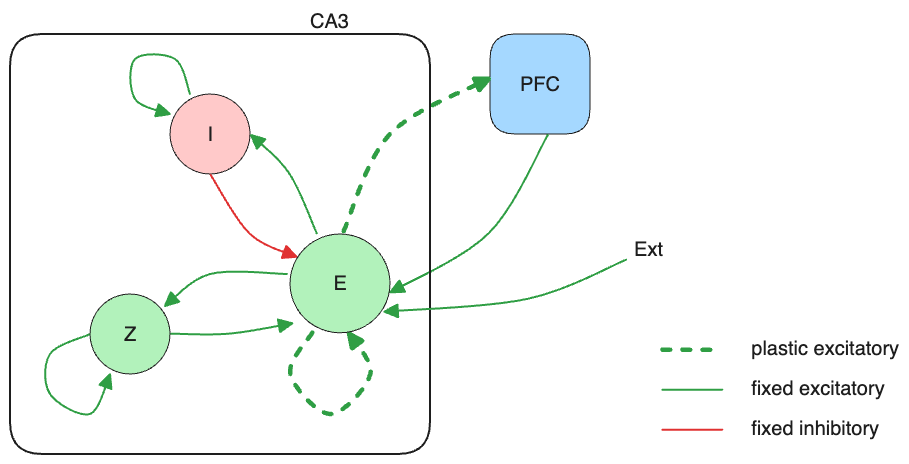
\includegraphics[width=0.6\textwidth]{figures/model_architecture_2.png}
%    \caption{\textsc{Model architecture - }\textit{$M$ is composed of three populations: excitatory (E), inhibitory (I) and auxiliary (Z), memory consolidation occurs only in the recurrent connection of population E. The $C$ is a mixed model, with a network and symbolic part, its afferent
%    connection from $M$ are plastic.}}
%    \label{fig:model_architecture1}
%\end{figure}


%% ------ HPC ------ %
%\hfill \break
%\noindent \textbf{Working Memory ($M$)}\\
%\noindent $M$ receives inputs from $C$ and from an external source, as illustrated in figure \ref{fig:model_architecture1} above. The external current is an aspecific spike input with a fixed rate of $300$Hz targeting all $M$'s neurons.
%The intent of this global excitation is to be strong enough to increase the activity in the recurrent network but also weak enough to allow drifts in the activity space influenced by the memory attractors. Then, $C$ stimulations further modulate the dynamics by providing a selective input to specific subnetworks. \\
%Another feature of $M$ is a working memory mechanism, which has the role of keeping active the neural pattern corresponding to the selected action (lever) and suppressing the others while waiting for the external feedback to arrive. This mechanism is implemented by a adding to the main
%excitatory population $E$ an inhibitory
%population $I$ and an auxiliary excitatory $Z$. The rationale behind this architecture is to have a way to bound the activity in $E$ through a proportional inihibition from $I$. However, when an attractor gets strong enough to meaningfully engage the population $Z$, which adds extra stimulation to
%the neurons involved in the memory, the inhibition $I$ silences effectively only the neurons not part of the active trace. \\
%% equations %
%The dynamics of $M$ are defined in terms of an internal variables $x^{\text{E}}_{t}$, which is the activity of the excitatory population $E$. In particular, the spiking behavour is described by a Spike Response Model (SRM) neuron model, which is based on a a series of kernels of the EPSP (and
%IPSP) for the relevant neuronal processes:
%\begin{equation}
%    \tau x^{E}_{i}=E_{\text{rest}}-x^{E}_{i}+\chi(t-t^{f}_{i}) + h^{EE}_{i} + h^{IE}_{i} + h^{ZE}_{i} + I^{\text{P}}_{i} + I^{\text{ext}}_{i}
%\end{equation}
%\noindent where $\chi$ is the kernel for the refractory period, $I^{\text{P}}_{i}$ is the projection from $C$, $I^{\text{ext}}_{i}$ is the external input, and $h^{EE}$ is the kernel for the recurrent connections, which define the contributions of spike trains $S^{E}_{j}$ from neighboring neurons:
%\begin{equation}
%    h^{EE}_{i}(t)=\sum\limits_{j}^{N^{E}}w_{ij}\int^{\infty}_{0}\kappa(s)S^{E}_{j}(t-s)ds
%\end{equation}
%\noindent where $\kappa$ is the synaptic kernel, and $w_{ij}$ is the synaptic weight for the recurrent connections $W^{EE}$. The kernels $h^{IE}$ and $h^{ZE}$ are defined similarly, but for the inhibitory and auxiliary populations, respectively. \\ The resulting spike train is then obtained by
%sampling from a Poisson process whose intensity is the non-linearly bounded internal variable:
%\begin{equation}
%    S_{i,t}\sim \mathcal{B}(\sigma_{\alpha, \beta}(x^{E}_{i}))
%\end{equation}
%\noindent where $\mathcal{B}$ is a Bernoulli sample, and $\sigma$ is a generalized sigmoid parametrized by $\alpha, \beta$. Each spike then updates, for each neuron $i$, its last spike-time $t^{f}_{i}$, used to calculate the EPSP in the SRM model.


%% ----- PFC ------ %

%\hfill \break
%\noindent \textbf{Executive Control ($C$)}\\
%\noindent $C$ receives afferent projections from $M$, which deliver the information about the currently active traces. Initially, these connections are set to zero, and $C$ is not influenced by $M$ activity, meaning it will settle for random decisions. Next, as the feedbacks start to accumulate,
%the afferent connections, which are plastic, get consolidated, encoding for a proxy of the value of the current option. \\
%$C$ defines its activity by means of a small neural network layer of leaky spiking neurons, which integrate the activity coming from $M$ and the an evaluation of the current options' value which can be considered a \textit{value function}, implemented through a non-linear function $\phi^{\text{P}}$:
%\begin{equation}
%    \tau \dot{u}^{\text{P}}_{i} = -u^{\text{P}}_{i} + \phi^{\text{P}}\left(W^{\text{HP}}_{i}\right)h^{\text{EP}}
%\end{equation}\label{pfc_x}
%From which the output is defined as follows:
%\begin{equation}
%    a_{i} = \text{relu}\left[\sigma_{\beta}\left(u_{i}\right) \mathcal{H}\left(h^{\text{EP}} - \theta_{1}\right)\right]
%\end{equation}
%\noindent where $\sigma_{\beta}$ is a generalized softmax parametrized by $\beta$, and $\mathcal{H}$ is the Heaviside function with threshold $\theta_{1}$.


%% ----- option selection ------ %

%% description of the model dynamics
%%\hfill  \break
%\subsubsection{Option selection}
%\noindent The decision making process is such that an output is well-defined only when $M$ is in a stable memory attractor that underlies an option that has also been selected by $C$. \\
%The excitatory population $E$ has around $\sim 50$ neurons for encoding each option, which has an average EPSP current $h^{\text{H}}_{k}$ ().where $\varphi_{K}$ is a function that compress the activity of the $N^{E}$ excitatory CA3 network into the vector of average activity for the traces $x^{\text{H}}_{t}$ of the $K$ memories.


%% ----- LEARNING ------ %

%\subsubsection{Learning rule}

%% - M - %
%In $M$, plasticity occurs only in the recurrent connections of the excitatory population $E$, with the scope of consolidating the memory traces. The synaptic weights are updated according to an Oja-style rule, that is dependent on the pre and post-synaptic activity, and on the current weight
%value. However, here it is introduced two modulation terms, $\text{DA}, \text{ACh}\in\{0,1\}$, which determines the direction of the update in either potentiation or depression respectively. The update in matrix form is given by:

%\begin{equation}
%    \Delta W^{\text{EE}} = \eta_{+}\text{DA}\,(W^{\text{EE}}_{\text{max}}-W^{\text{EE}})\,\Delta^{\text{hebb}} - \eta_{-}\text{ACh}\,W^{\text{EE}}\,\Delta^{\text{hebb}}
%\end{equation}

%\noindent where $\eta_{+}, \eta_{-}$ are the learning rates, and $W^{\text{EE}}_{\text{max}}$ is the maximum weight value. The Hebbian term $\Delta^{\text{hebb}}$ is calculated through a Gaussian filter with width $\tau_{\text{ps}}$ and shape $\phi(t)=e^{-0.5\,(\frac{t}{\tau_{\text{ps}}})^2}$ over the time of the last spike of the pre and post-synaptic neurons $i,j$:
%\begin{equation}
%    \Delta^{\text{hebb}}_{ij} = \phi(t-\mathbf{t}^{f}_{i})\,\phi(t-\mathbf{t}^{f}_{j})^{T}
%\end{equation}

%\noindent Then, for homeostatic reasons, the weights are clipped in $\left(0, W^{\text{EE}}_{\text{max}}\right)$ and normalized such that the total input remains constant $w_i=\bar{w}^{EE}\,\frac{w_i}{\sum\limits_{j}w_{ij}}$.

%\hfill \break
%% - PFC - %
%As for the $C$, learning happens in the afferent projections from $M$, with the intent of encoding the value of the currently active option. As before, the update is dependent on the valence of the feedback, gated by the dopamine and acetylcholine signals. However, unlike $M$, the specific rule
%is defined only in terms of the pre-synaptic activity and the current weight value, and it takes the form of a mixture of Gaussians $\Theta_{\pm}$, with different parameters for potentiation and depression respectively. The update is given by:
%\begin{equation}
%    \Delta W^{\text{HP}} = \eta\,\phi(t-\mathbf{t}^{f})\,\left[\text{DA}\,\Theta_{+}(W^{\text{HP}}) - \text{ACh}\,\Theta_{-}(W^{\text{HP}})\right]
%\end{equation}

%\noindent where $\textbf{t}^{f}$ is the time of the last spike of the pre-synaptic neuron, and $\eta$ is the learning rate.


%% ----- OPTIMIZATION ------ %

%\subsubsection{Performance}

%\noindent Given the model architecture, the performance of the agent is significantly determined by the $C$ dynamics, which biases the $M$ activity to pivot towards a preferred option. In particular, the shape of the $C$'s synaptic plasticity function $\Theta_{\pm}$ enables a non-linear
%consolidation of the afferent connections and a specific rate of change for potentiation and depression, with the scope of differentiating between small, medium, and large weights. Similarly, the non-linearity of the \textit{value function} $\phi^{\text{P}}$ is crucial in determining the influence
%on the $M$ activity while considering the current evaluation of the options. \\
%Both the synaptic plasticity function and the value function are implemented as a mixiture of Gaussians:

%\begin{equation}
%\phi_{2}(x)=r\,\gamma_{1}\exp\left[-\left(\frac{x-\mu_1}{\sigma_{1}}\right)^{2}\right]+(1-r)\,\gamma_{2}\exp\left[-\left(\frac{x-\mu_2}{\sigma_{2}}\right)^{2}\right]
%\end{equation}
%with function-specific parameters: $\{r, \gamma_{1}, \gamma_{2}, \mu_{1}, \mu_{2}, \sigma_{1},\sigma_{2}\}$.

%\hfill \break
%The optimization of the parameters has been carried out through an evolutionary search using the Covariance Matrix Adaptation Evolution Strategy (CMA-ES) algorithm, which is a stochastic optimization method particularly suited for high-dimensional and non-linear optimization problems. 

